\section{Langkah-Langkah Percobaan}
1. Konfigurasi DHCP Client pada Router A (Ether 1), sambungkan kabel internet ke ether1 pada Router A, kemudian lakukan konfigurasi DHCP Client. \\
2. Penambahan Alamat IP pada Ether 7, Tambahkan alamat IP pada ether7 untuk konektivitas dengan Switch. Masukkan Address: 192.168.10.1/24.
\begin{figure}[H]
    \centering
    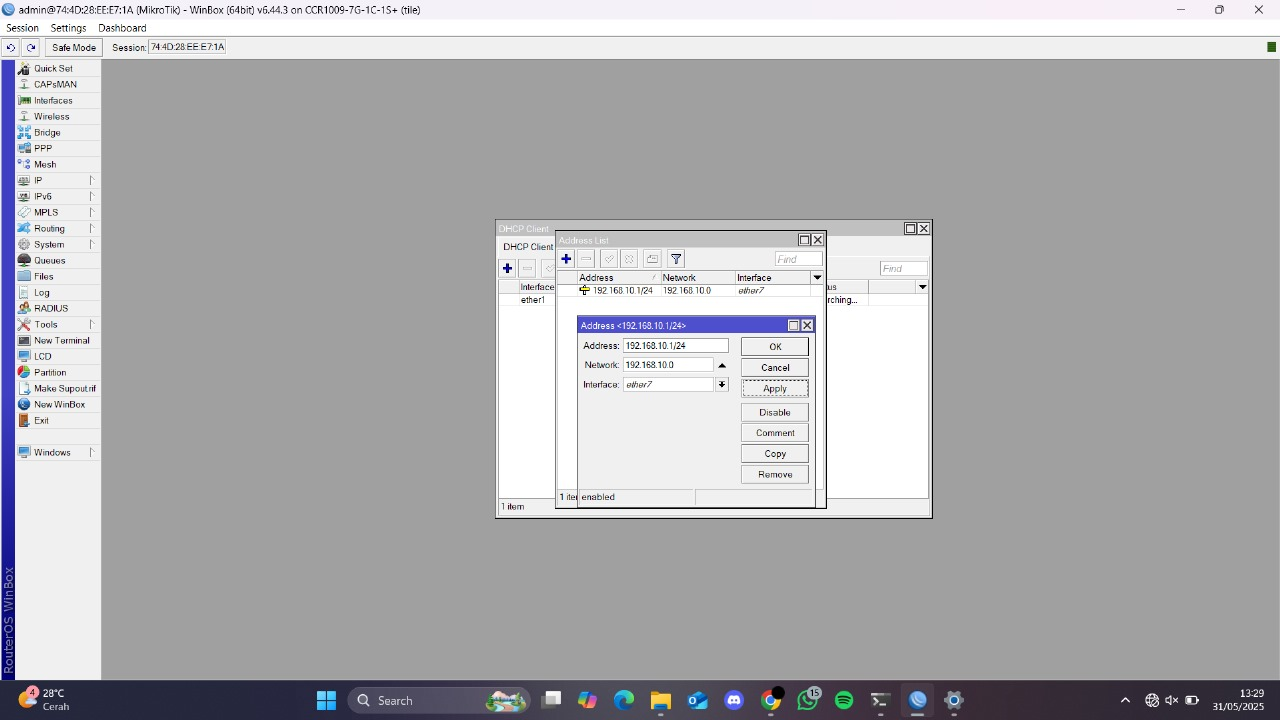
\includegraphics[width=0.65\linewidth]{image/clnt1.jpg}
    \label{fig:inirujukan}
    \caption{Konfigurasi DHCP client dan Ip address ether 7}
\end{figure}
3. Konfigurasi DHCP Server pada Router MikroTik. Konfigurasi DHCP Server untuk secara otomatis mendistribusikan alamat IP kepada perangkat klien yang terhubung.
\begin{figure}[H]
    \centering
    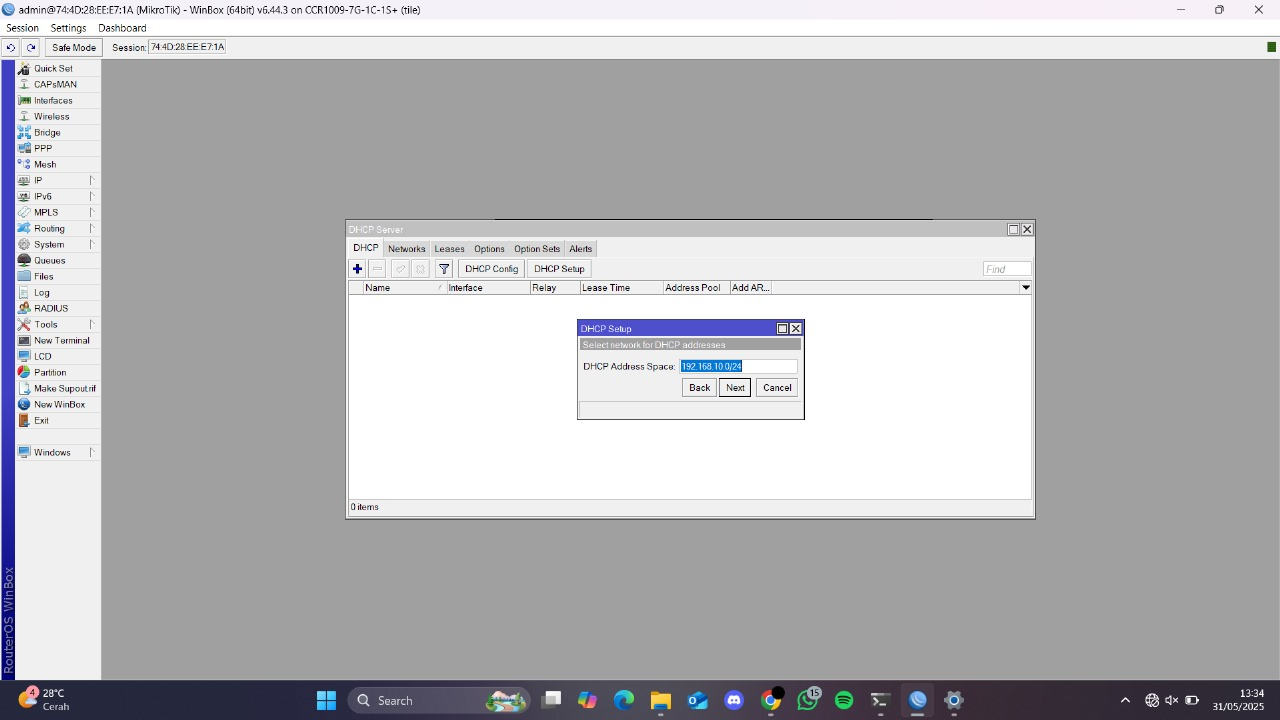
\includegraphics[width=0.65\linewidth]{image/clnt2.jpg}
    \label{fig:inirujukan}
    \caption{Konfigurasi DHCP server}
\end{figure}
4. Konfigurasi NAT. Lakukan konfigurasi NAT (Network Address Translation) untuk menyediakan konektivitas internet.
\begin{figure}[H]
    \centering
    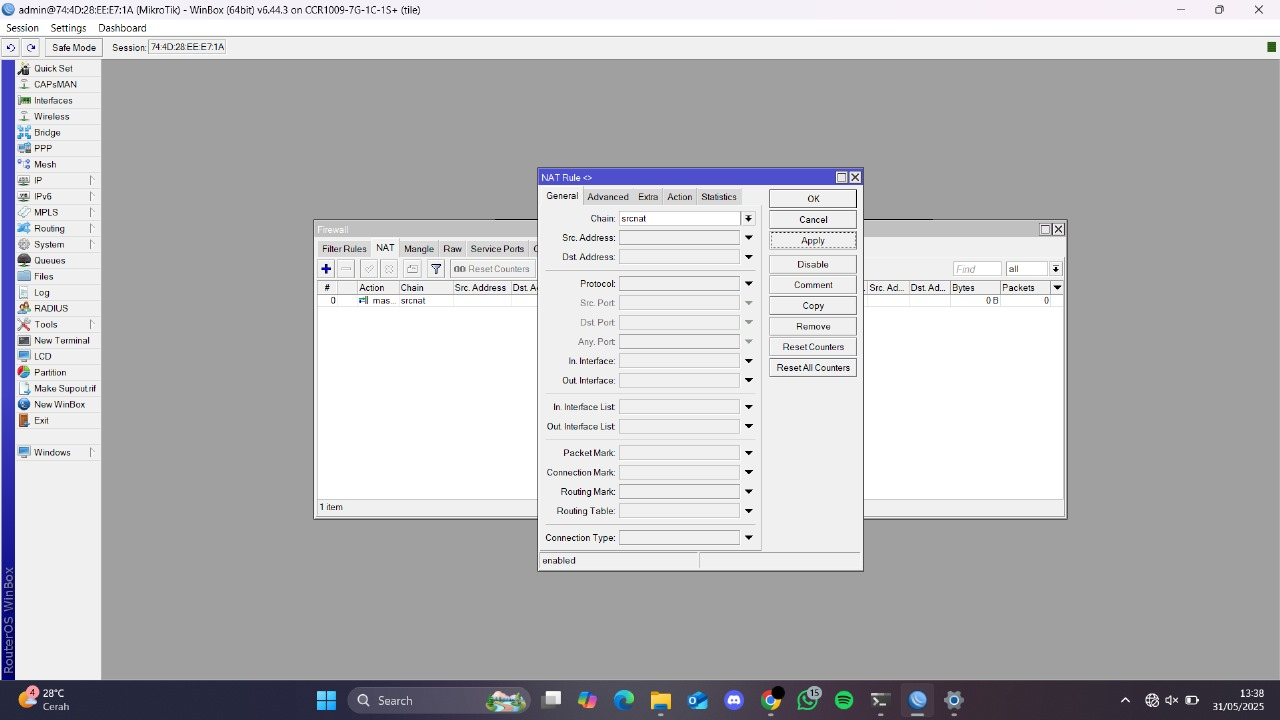
\includegraphics[width=0.65\linewidth]{image/clnt3.jpg}
    \label{fig:inirujukan}
    \caption{Konfigurasi NAT}
\end{figure}
5. Konfigurasi Firewall. Tambahkan aturan filter (Filter Rules) pada firewall.
\begin{figure}[H]
    \centering
    \begin{subfigure}[b]{0.3\linewidth}
      \centering
      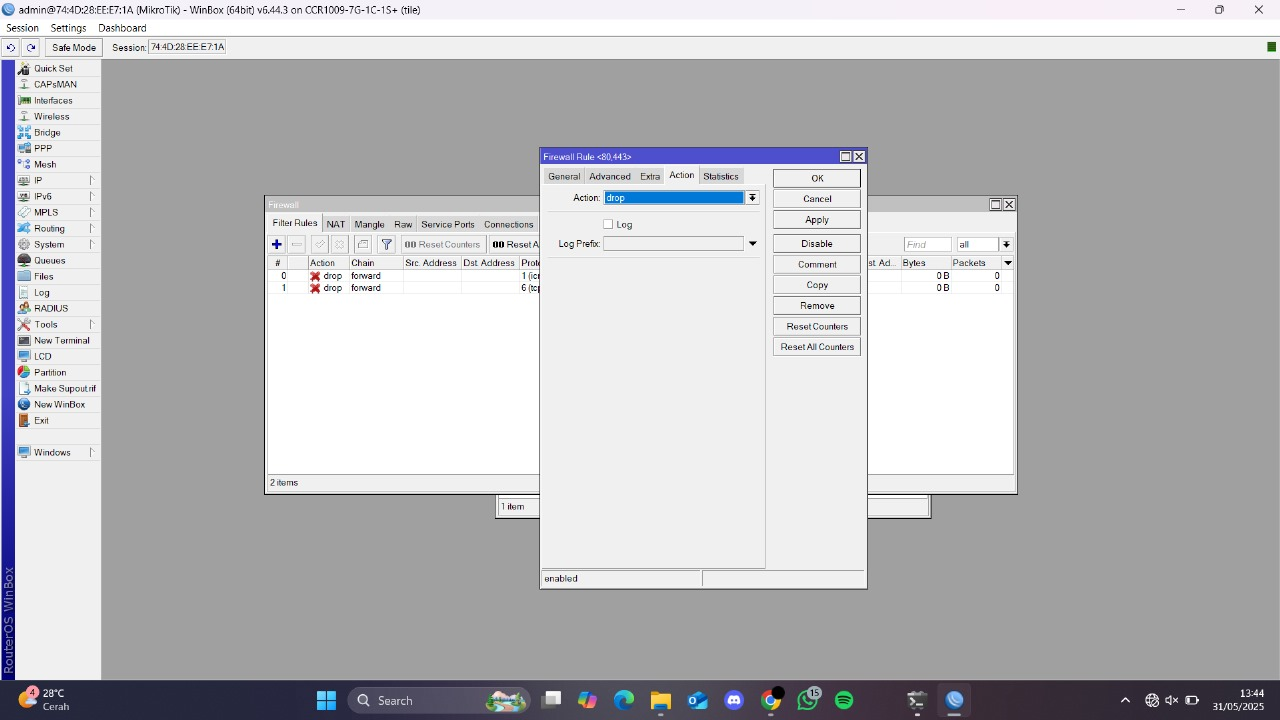
\includegraphics[width=\linewidth]{image/clnt4.jpg}
    \end{subfigure}
    \hspace{1cm}
    \begin{subfigure}[b]{0.3\linewidth}
      \centering
      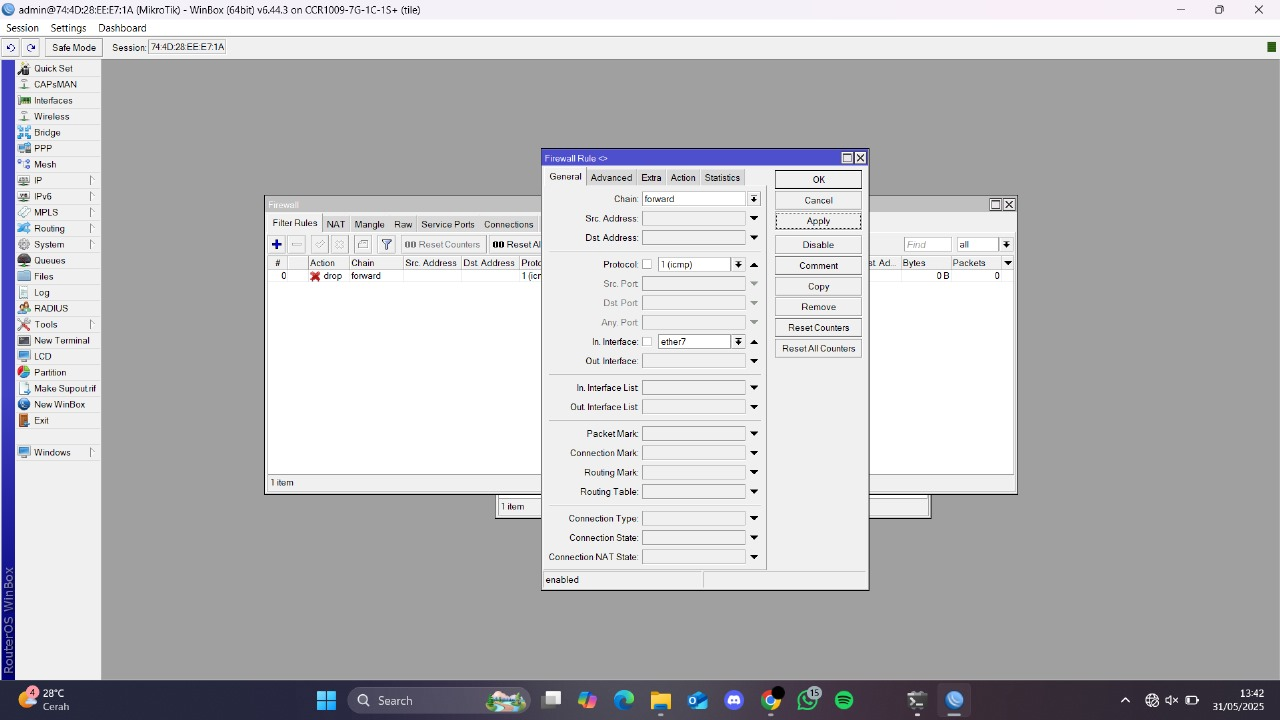
\includegraphics[width=\linewidth]{image/clnt5.jpg}
    \end{subfigure}
    \begin{subfigure}[b]{0.3\linewidth}
      \centering
      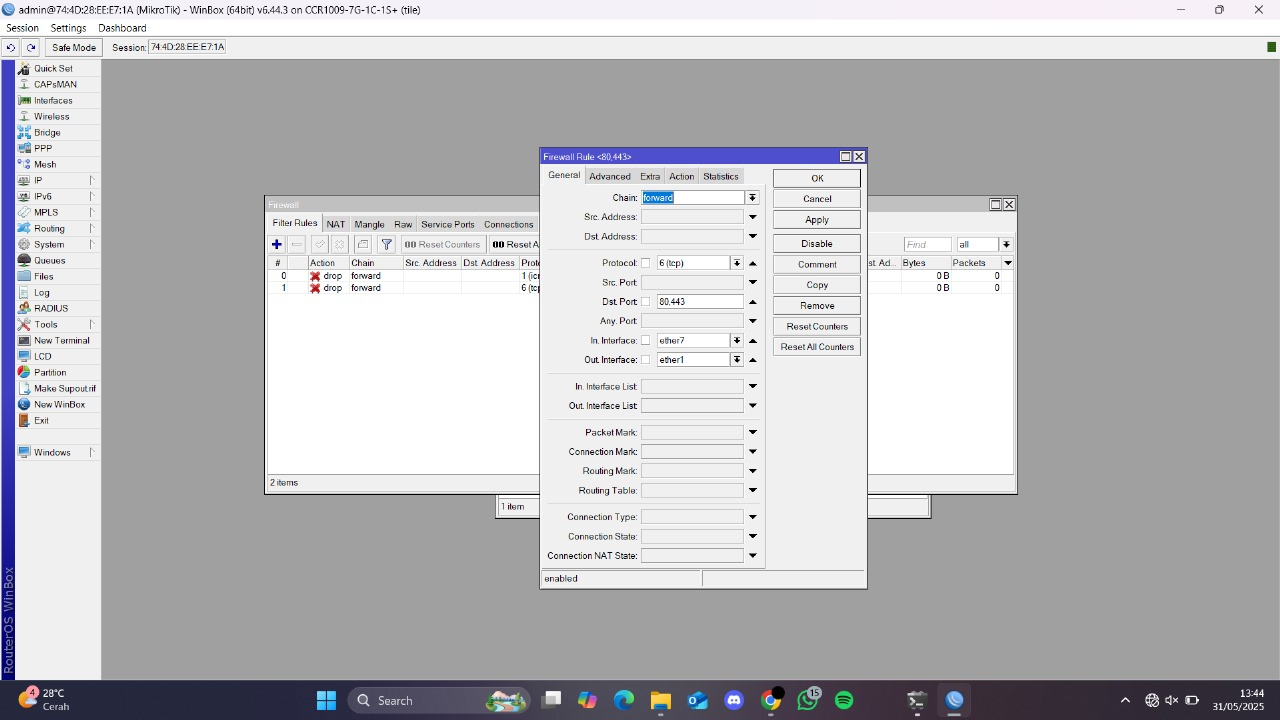
\includegraphics[width=\linewidth]{image/clnt6.jpg}
    \end{subfigure}
    \hspace{1cm}
    \begin{subfigure}[b]{0.3\linewidth}
      \centering
      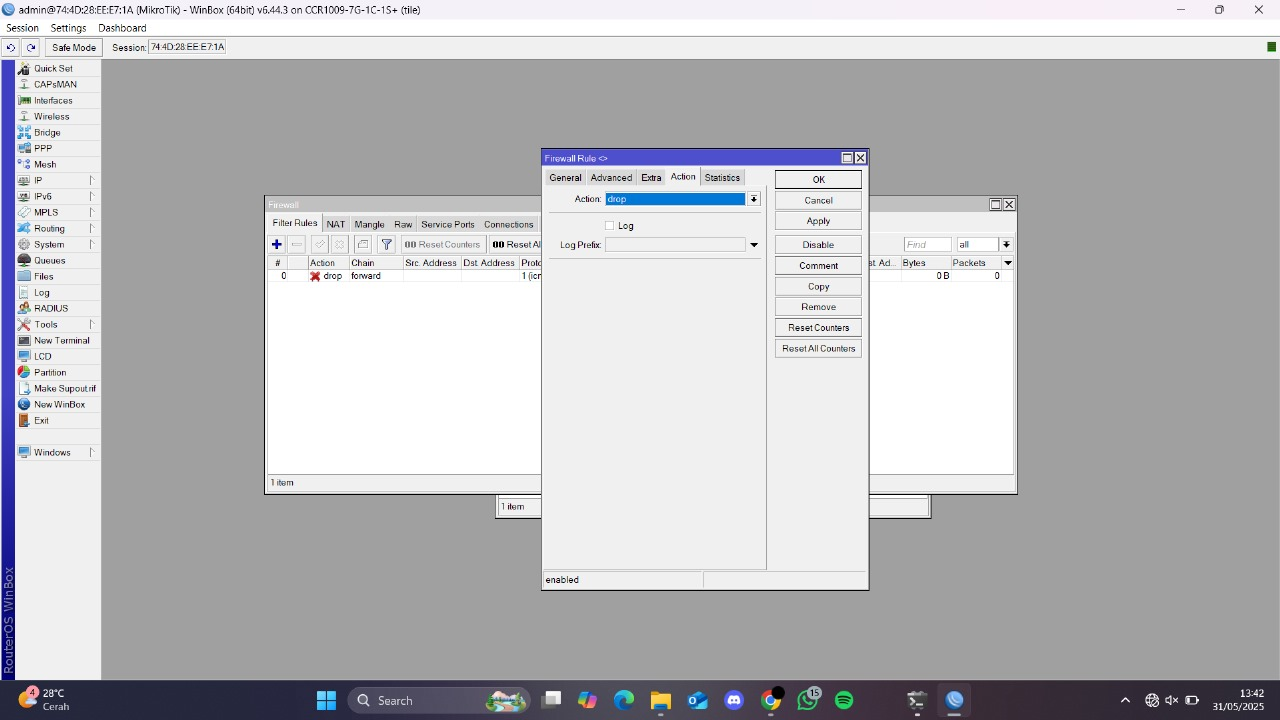
\includegraphics[width=\linewidth]{image/clnt7.jpg}
    \end{subfigure}
    \caption{Konfigurasi firewall}
\end{figure}
6. Konfigurasi Bridge pada Router B. Lakukan konfigurasi bridge untuk mengubah fungsi Router B menjadi hub. Selanjutnya, tambahkan port ke dalam bridge yang telah dibuat.
\begin{figure}[H]
    \centering
    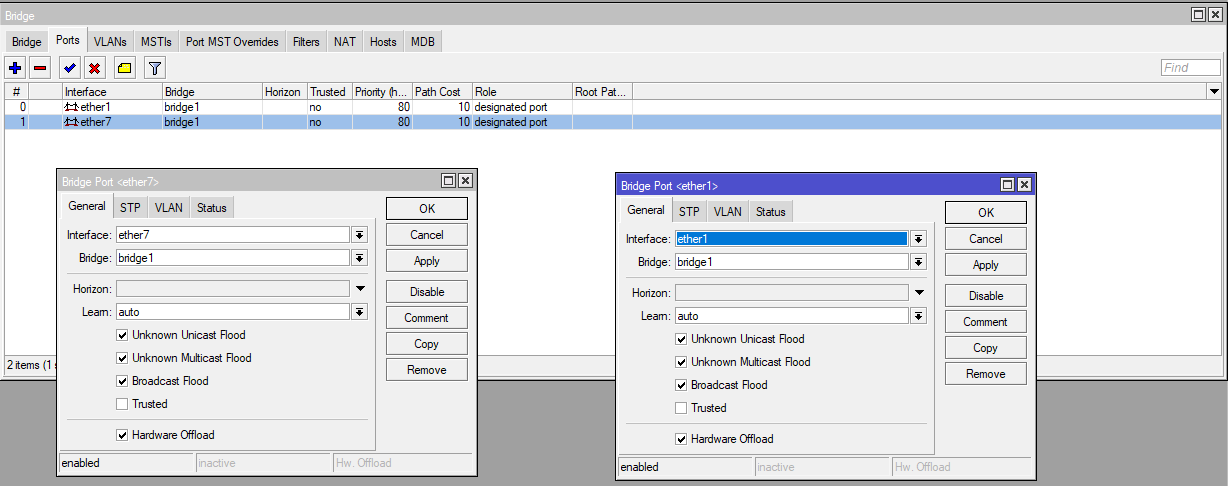
\includegraphics[width=0.65\linewidth]{image/bdg2.png}
    \label{fig:inirujukan}
    \caption{Konfigurasi bridge}
\end{figure}
7. Konfigurasi Alamat IP pada Laptop. Pastikan pengaturan alamat IP pada laptop diatur secara otomatis melalui DHCP, lalu verifikasi perolehan alamat IP.
\begin{figure}[H]
    \centering
    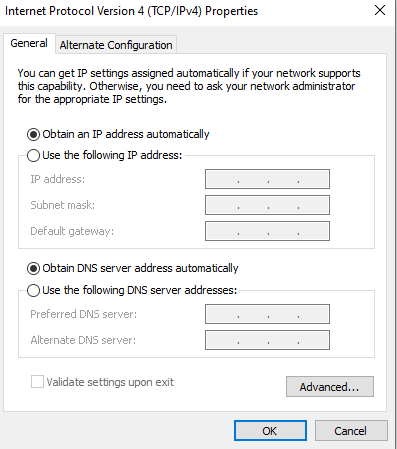
\includegraphics[width=0.65\linewidth]{image/bdg3.png}
    \label{fig:inirujukan}
    \caption{Konfigurasi IP pada laptop}
\end{figure}
8. Uji Coba Konfigurasi. Lakukan pengujian terhadap konfigurasi yang telah diterapkan untuk memverifikasi fungsionalitasnya. Pengujian Konektivitas (ICMP): ping 8.8.8.8. Pengujian Pemblokiran Konten (Browse): akses speedtest.net. 
\begin{figure}[H]
    \centering
    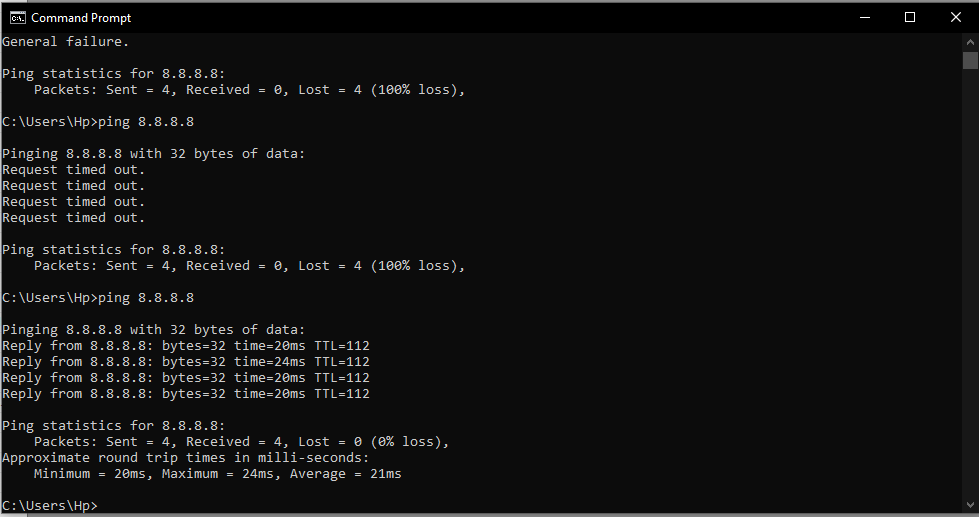
\includegraphics[width=0.65\linewidth]{image/bdg4.png}
    \label{fig:inirujukan}
    \caption{tes ping pada cmd}
\end{figure}
\begin{figure}[H]
    \centering
    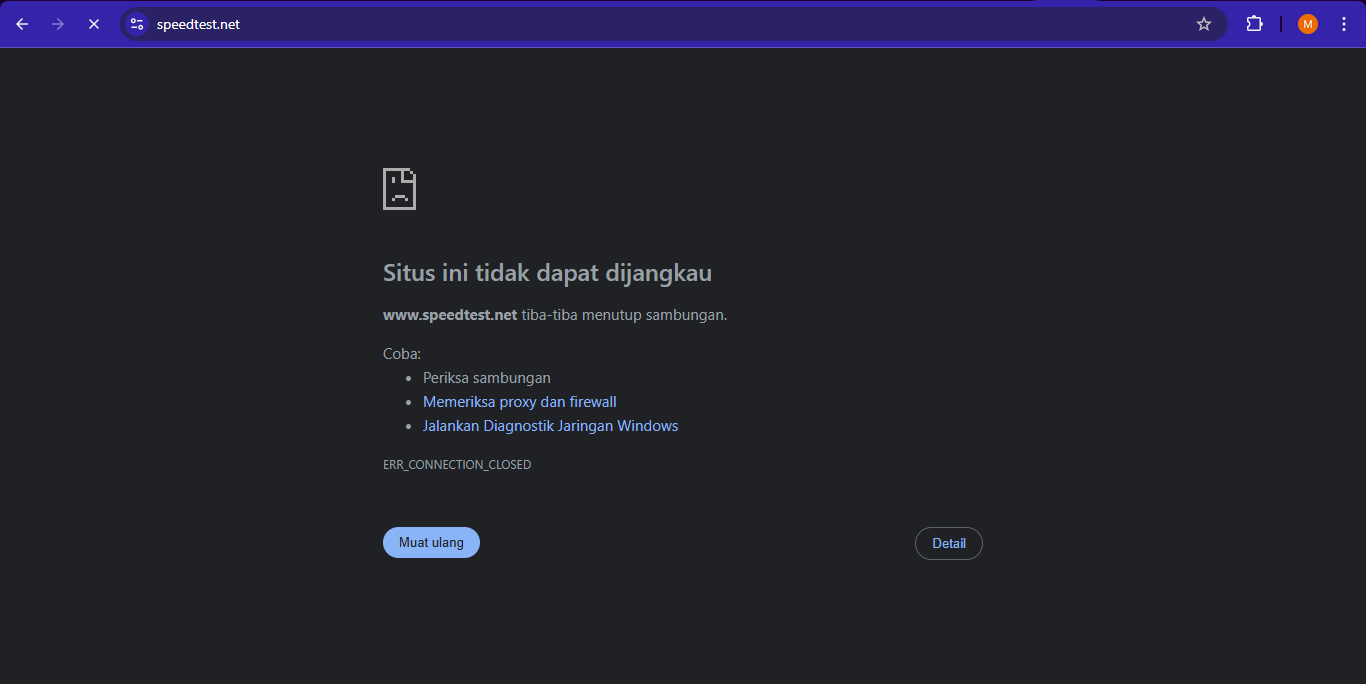
\includegraphics[width=0.65\linewidth]{image/bdg5.png}
    \label{fig:inirujukan}
    \caption{saat firewall dinyalakan}
\end{figure}
\begin{figure}[H]
    \centering
    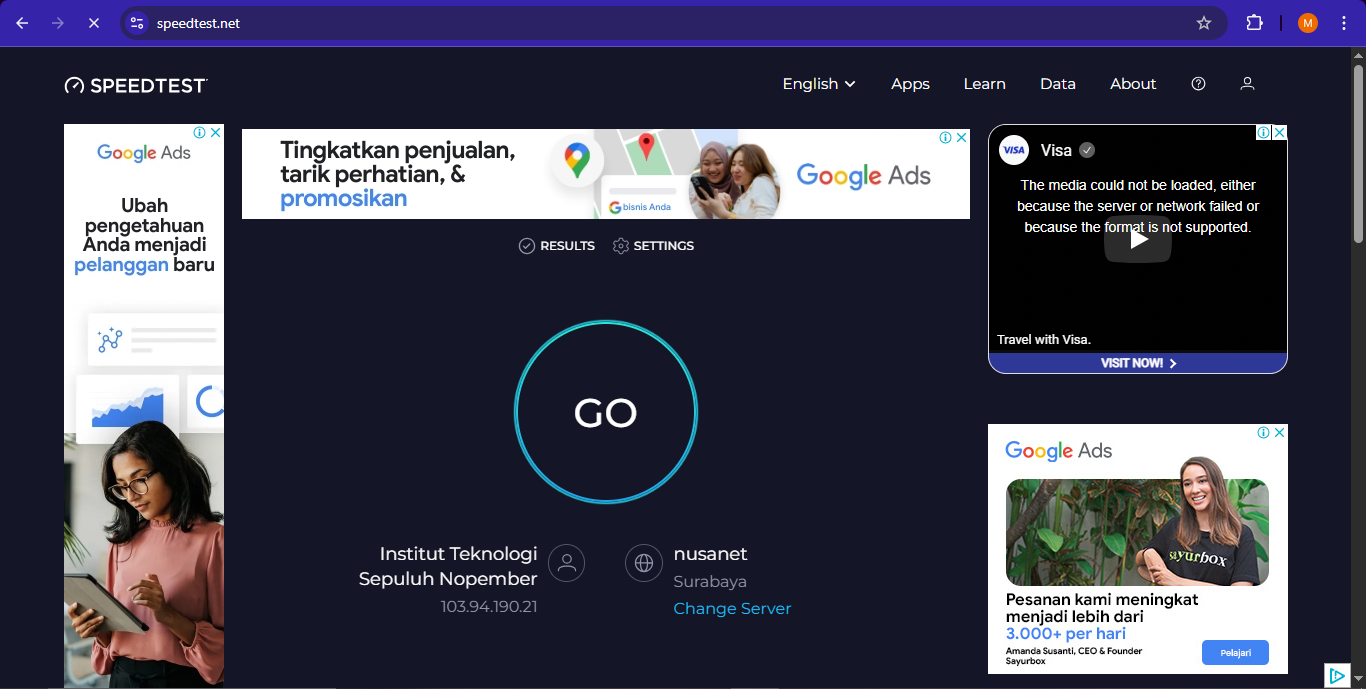
\includegraphics[width=0.65\linewidth]{image/bdg6.png}
    \label{fig:inirujukan}
    \caption{saat firewall dimatikan}
\end{figure}

\section{Analisis Hasil Percobaan}
Selama praktikum konfigurasi Firewall dan NAT menggunakan perangkat MikroTik, dilakukan beberapa tahapan pengujian untuk memastikan fungsi dasar jaringan dan keamanannya berjalan sesuai teori. Tahapan pertama adalah konfigurasi DHCP, di mana router berhasil mendistribusikan alamat IP secara otomatis ke laptop melalui interface ether7. Laptop memperoleh IP dalam rentang 192.168.10.2–192.168.10.254, sesuai dengan teori DHCP Server yang memungkinkan pemberian alamat IP dinamis. Tidak ada kendala berarti selama proses ini, yang menunjukkan bahwa layanan DHCP pada MikroTik berfungsi dengan baik, meskipun potensi kegagalan bisa terjadi jika pemilihan interface tidak tepat. \\ Pada konfigurasi NAT (Network Address Translation), laptop dapat melakukan ping ke alamat IP 8.8.8.8 setelah aturan masquerade diterapkan. Hal ini menunjukkan bahwa NAT bekerja sesuai teori, khususnya jenis Port Address Translation (PAT), yang memungkinkan beberapa IP lokal berbagi satu IP publik untuk mengakses internet. Kegagalan pada tahap ini umumnya disebabkan oleh kesalahan konfigurasi pada interface atau pengaturan yang tidak di-apply dengan benar. \\ Selanjutnya, pengujian firewall untuk pemblokiran ICMP menunjukkan hasil yang sesuai dengan ekspektasi. Saat aturan firewall diaktifkan, perintah ping dari laptop ke internet tidak mendapat balasan (Request Timed Out), dan saat aturan dinonaktifkan, koneksi kembali normal. Hal ini membuktikan bahwa firewall berfungsi sebagai filter lalu lintas data dan mematuhi aturan yang ditentukan. \\ Pengujian lanjutan dilakukan untuk filtering konten dengan kata kunci “speedtest”. Saat aturan aktif, situs seperti speedtest.net tidak dapat diakses, dan kembali normal setelah aturan dinonaktifkan. Ini menunjukkan bahwa firewall mampu melakukan filtering berbasis konten pada protokol HTTP. Namun, filtering konten memiliki keterbatasan ketika berhadapan dengan situs yang sepenuhnya menggunakan HTTPS karena enkripsi data menyulitkan firewall untuk membaca isi paket. \\ Pada tahap terakhir, Router B dikonfigurasi sebagai bridge untuk mengubahnya menjadi switch yang memungkinkan distribusi koneksi ke beberapa perangkat. Konfigurasi berhasil dan sesuai prinsip switching pada layer 2. Kendala yang mungkin terjadi adalah kelalaian dalam menambahkan port ke dalam bridge atau tidak menonaktifkan IP statis pada Router B, yang bisa menyebabkan konflik jaringan.

\section{Hasil Tugas Modul}
\begin{figure}[H]
    \centering
    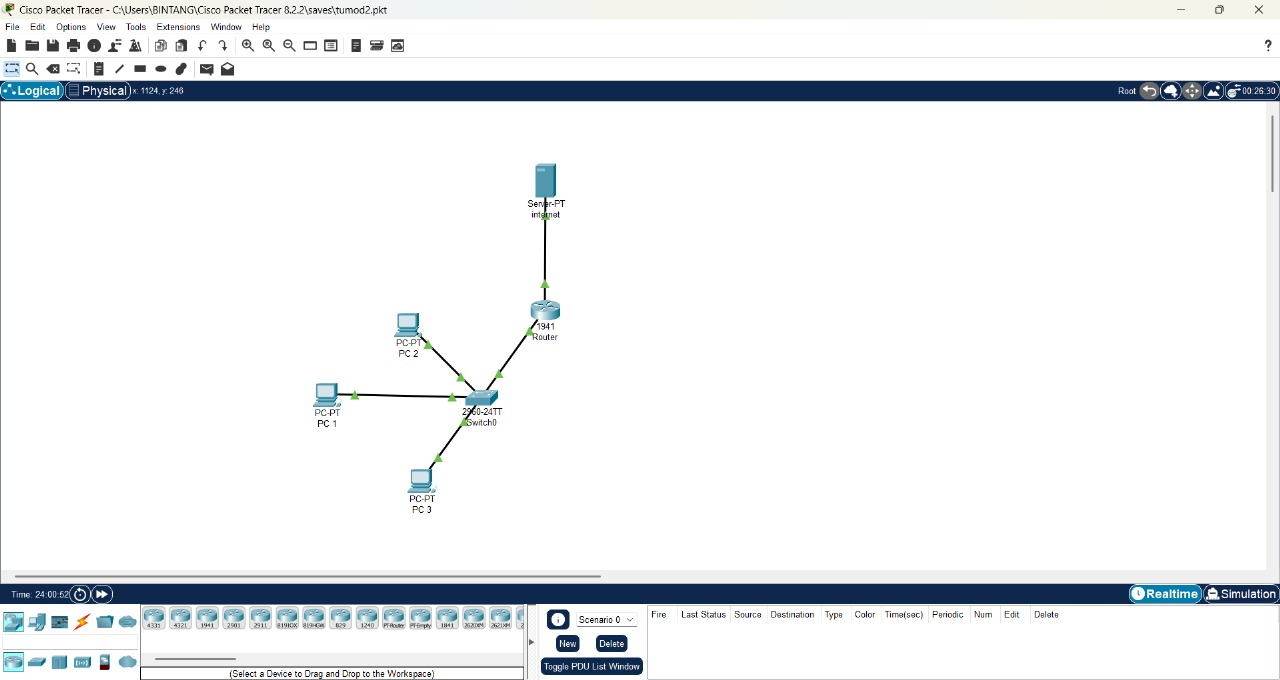
\includegraphics[width=0.65\linewidth]{image/tumod.jpg}
    \label{fig:inirujukan}
    \caption{hasil tugas modul}
\end{figure}
\subsection {Hasil konfigurasi Ip address} 
- Router (LAN side): 192.168.1.1/24 \\ 
- Router (WAN side): 200.200.200.1/24 \\
- Server (Public): 200.200.200.2/24 \\
- PC1: 192.168.1.2/24 \\
- PC2: 192.168.1.3/24 \\
- PC3: 192.168.1.4/24 \\
- Gateway ketiga PC: 192.168.1.1
\subsection{Konfigurasi NAT}
Masuk ke CLI : \\
\# interface FastEthernet0/0 \\
 ip address 192.168.1.1 255.255.255.0 \\
 ip nat inside \\
 no shutdown \\
\# interface FastEthernet0/1 \\
 ip address 200.200.200.1 255.255.255.0 \\
 ip nat outside \\
 no shutdown \\
 ip nat inside source list 1 interface FastEthernet0/1 overload. \\
 access-list 1 permit 192.168.1.0 0.0.0.255
\subsection{Konfigurasi Firewall (ACL)}
Tujuan : \\
- Hanya PC2 yang boleh akses server. \\
- PC1 dan PC3 diblokir dari akses server. \\
- Semua PC tetap bisa komunikasi antar sesama di LAN. \\ \\ 
Langkah : \\
access-list 100 permit ip 192.168.1.3 0.0.0.0 host 200.200.200.2 \\
access-list 100 deny ip 192.168.1.2 0.0.0.0 host 200.200.200.2 \\
access-list 100 deny ip 192.168.1.4 0.0.0.0 host 200.200.200.2 \\
access-list 100 permit ip any any \\
ACL yang mengarah ke server : \\
interface FastEthernet0/1 \\
 ip access-group 100 out

\section{Kesimpulan}
Praktikum ini bertujuan untuk memberikan pemahaman langsung kepada praktikan mengenai penerapan Network Address Translation (NAT) dan Firewall pada perangkat jaringan. \\ Hasil yang diperoleh menunjukkan bahwa konfigurasi DHCP berhasil mendistribusikan alamat IP secara otomatis kepada perangkat klien. NAT berfungsi sebagaimana mestinya dengan memungkinkan seluruh perangkat dalam jaringan lokal mengakses internet melalui satu IP publik. Sementara itu, firewall juga berjalan dengan baik; baik untuk memblokir koneksi ICMP maupun konten tertentu berbasis HTTP. Pengujian terhadap filtering akses berdasarkan alamat IP dan port pada Cisco Packet Tracer juga membuktikan bahwa Access Control List (ACL) dapat digunakan untuk membatasi akses tertentu secara selektif. \\ Secara keseluruhan, hasil praktikum ini sesuai dengan teori yang telah dipelajari. Praktikan dapat memahami perbedaan jenis-jenis firewall, jenis-jenis NAT, serta bagaimana konfigurasi koneksi dapat memengaruhi lalu lintas jaringan. Selain itu, praktikum ini menekankan pentingnya ketelitian dalam memilih interface, chain, dan parameter saat mengatur rule di router.

\section{Lampiran}
\begin{figure}[H]
    \centering
    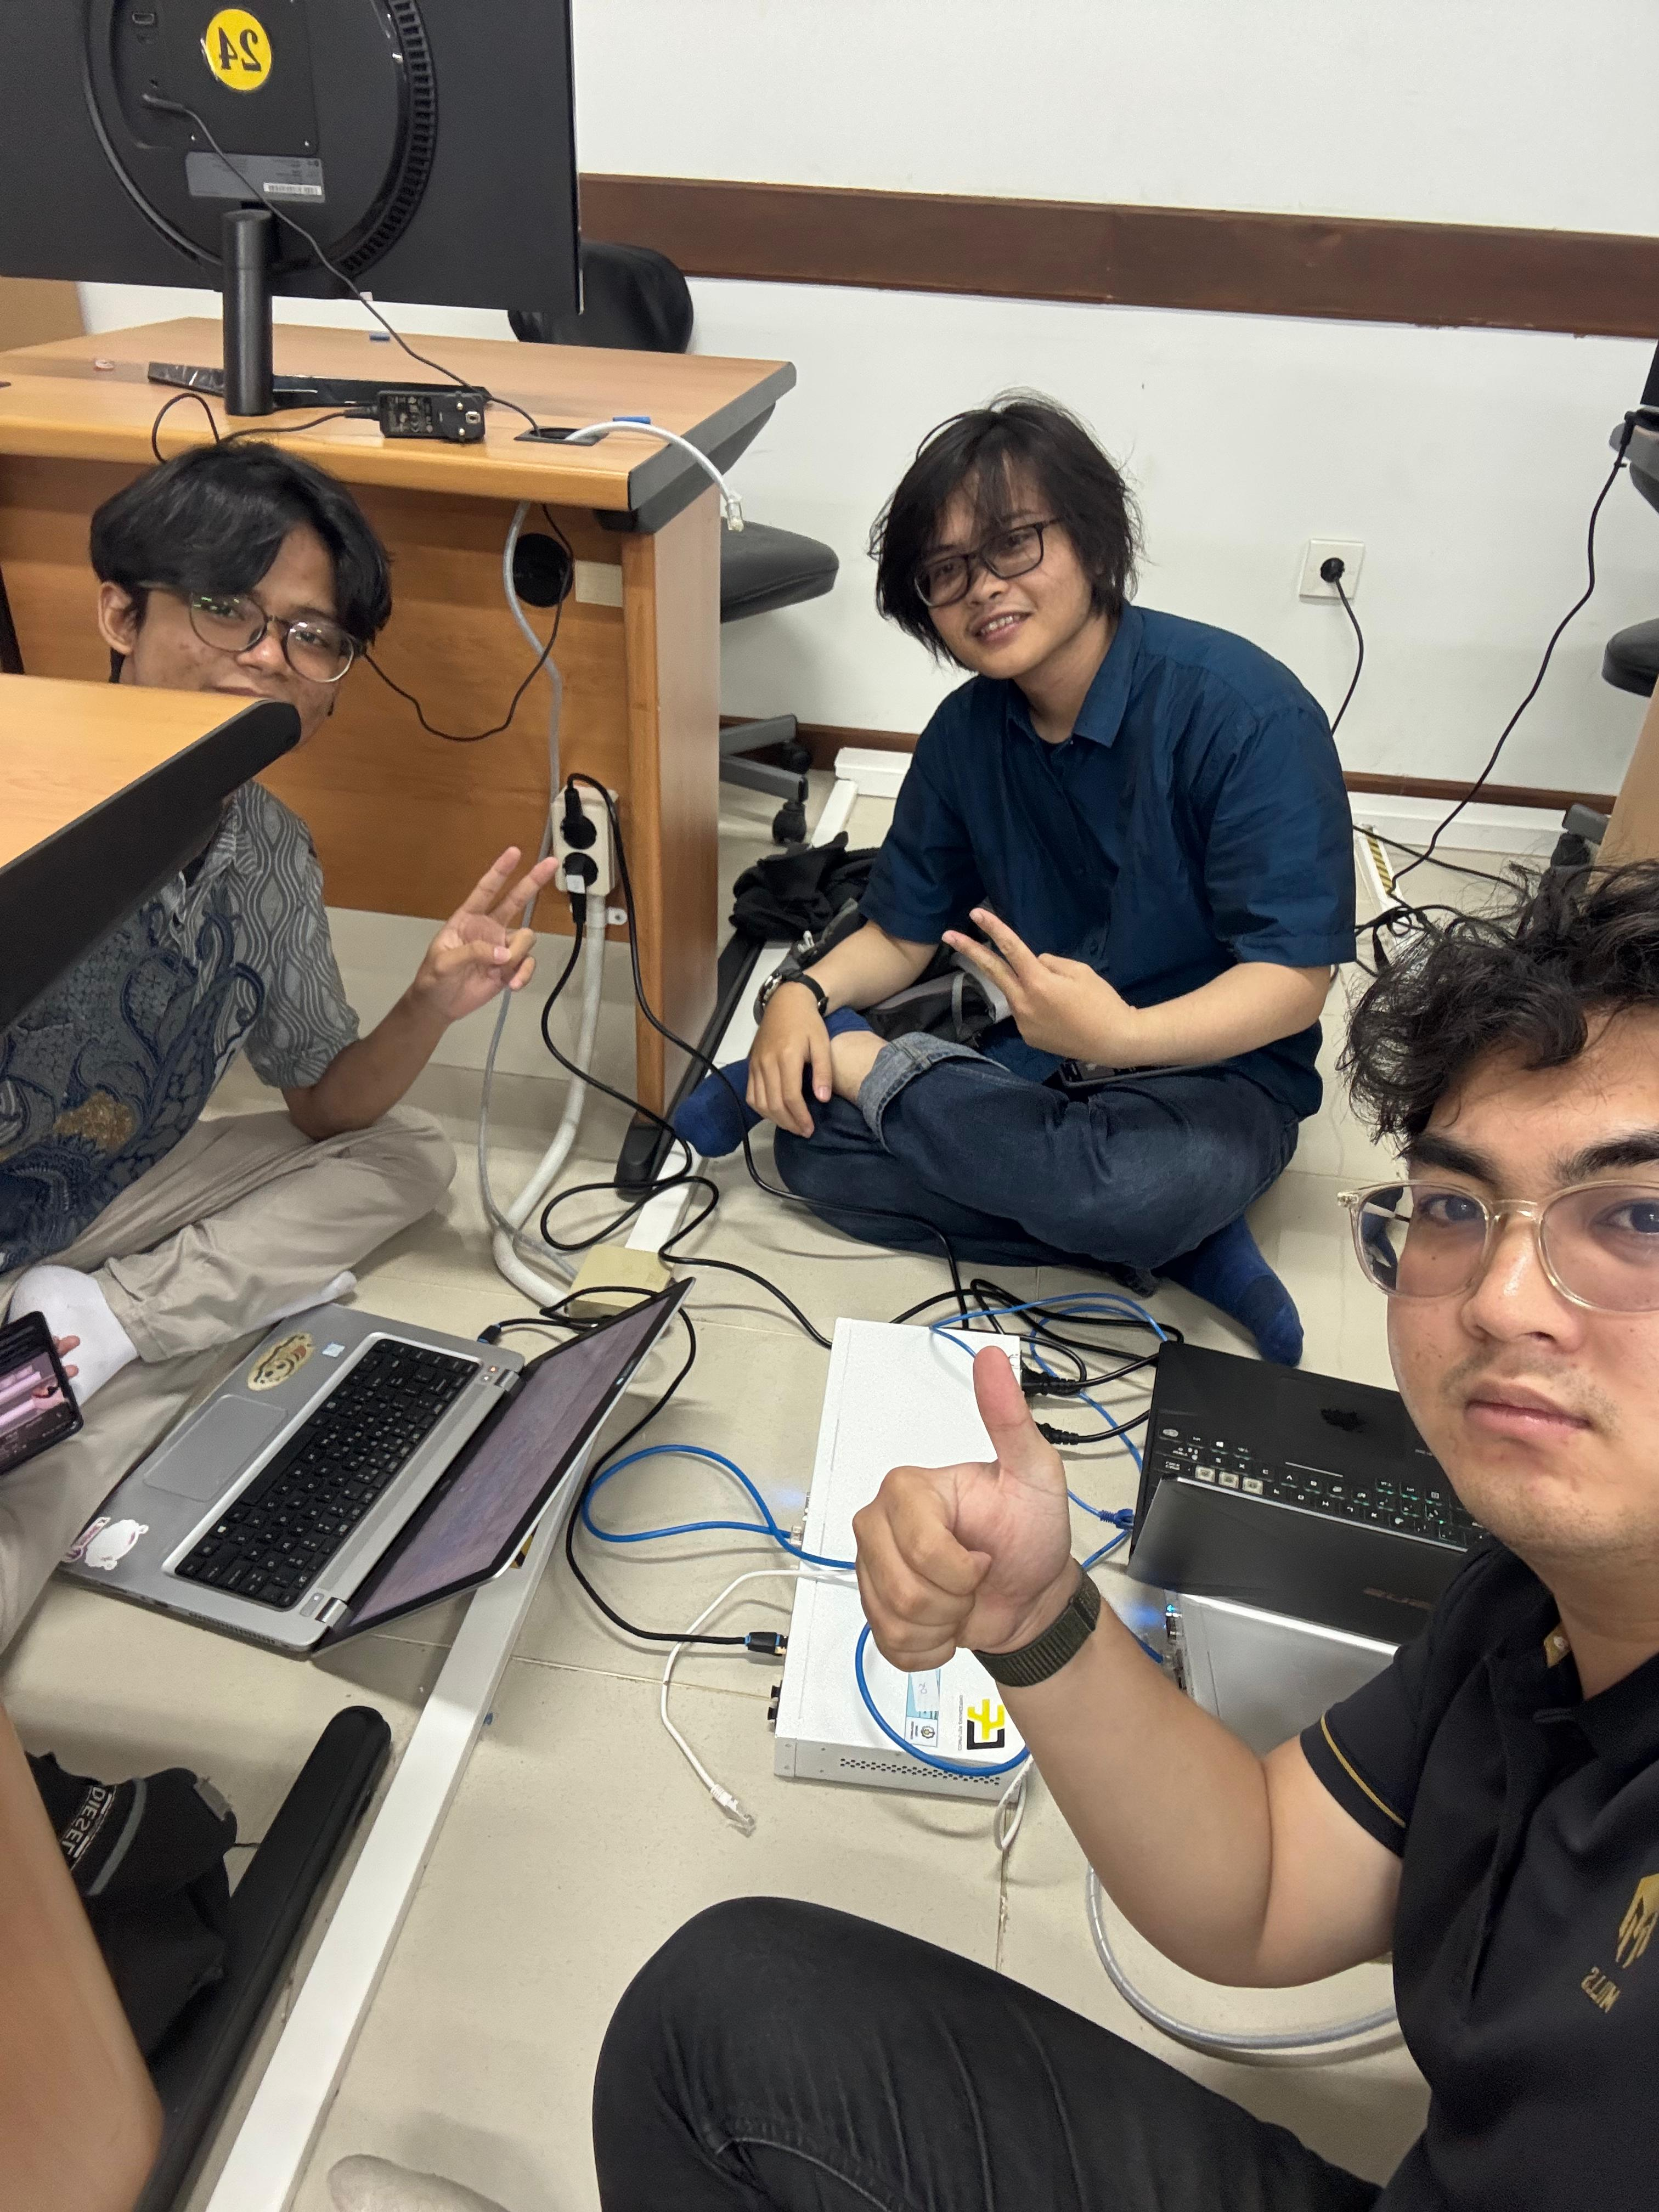
\includegraphics[width=0.65\linewidth]{image/dokum.jpg}
\end{figure}
